% Chapter mh: Maslanka, Haglund and the missing positivity. Sources: misc/reviews/nick-maslanka-haglund/maslanka_haglund_for_vadim/maslanka_haglund_chapter.tex (whole draft), referee report MH (M1 to M9), verification misc/vol3/verify/MH/results.md; edited 17 Nov 2026 (final text 19 Nov 2026).
\label{mh:ch:maslanka}
The positive Maslanka criterion of the preceding chapter (Theorem~\ref{cw:thm:maslanka}, with the Williamson densities of Proposition~\ref{cw:prop:williamson}) concerns the positive sequence $d_k$ built from the primes. This chapter writes the same sequence for $\xi$ itself, where the pole and the trivial zeros are absorbed by the Gamma factor, and the sequence becomes a pure sum over the zeros: a linear statistic of the Thorin measure $U_{1/2}=\sum_{\gamma>0}\delta_{\gamma^2}$ with Beta kernels (Theorem~\ref{mh:thm:zerosum}). RH is equivalent to a one sided bound on it (Theorem~\ref{mh:thm:landau}). The $2\sin^2$ lemma gives a bound of the right kind but of order $k^{-1/2}$ where $k^{-3/4}$ is needed (Proposition~\ref{mh:prop:sin2}). The second half asks whether Haglund's incomplete gamma identity for $\Xi$ lends itself to Wald couples, van Dantzig pairs or the Thorin approach. The identity is a positive mixture, but each component has a kink at the origin, which is the mechanism of Chapter~\ref{ch:miyatake}. The Wald partner of $\Xi$ exists with no hypothesis (Proposition~\ref{c:thm:wald}), and Section~\ref{mh:sec:tolerance} shows how much off line mass complete monotonicity tolerates, which is why existence of the partner cannot separate $\zeta$ from a function that only behaves like it. Section~\ref{mh:sec:ladder} gives the Hankel form of the total positivity ladder and a table of planted off line pairs. The new material is from an unrefereed note of Polson (November 2026). Throughout, $\Theta=\sup\Re\rho$ over the nontrivial zeros, so that $\Theta\le\frac78$ by the theorem of \cite{OAI26a}, and RH is $\Theta=\frac12$.

\section{The Ma\'slanka sequence of $\xi$}\label{mh:sec:zerosum}

Let $\xi(s)=(s-1)\pi^{-s/2}\Gamma(\tfrac s2+1)\zeta(s)$, which is $\frac12s(s-1)\pi^{-s/2}\Gamma(\frac s2)\zeta(s)$, and $G=\xi'/\xi$. Put $d_k=\sum_n\Lambda(n)n^{-2}(1-n^{-2})^k$ and $R_k=d_k-\tfrac12B(\tfrac12,k+1)$, the positive sequence and its remainder of the preceding chapter. Maslanka's own coefficients are the binomial differences $A_k$ of $(2j+1)\zeta(2j+2)$ of Proposition~\ref{prop:ch19:maslanka} \cite{Maslanka01,BaezDuarte10}. The sequence below is the analogous binomial difference of $G$ at the even integers, and we call it the Maslanka sequence of $\xi$ by that analogy only. Define
\[
g_k=\sum_{j=0}^k(-1)^j\binom kj\,G(2j+2).
\]

\begin{theorem}\label{mh:thm:zerosum}
For $k\ge1$,
\[
g_k=\tfrac12\sum_\rho B\big(1-\tfrac\rho2,k+1\big)=-R_k-\frac{1}{2k(k+1)} ,
\]
the sum converging absolutely. Further $g_k=O(k^{-1+\Theta/2})$, so $g_k=O(k^{-9/16})$ unconditionally by \cite{OAI26a}, and
\[
G(2-2z)=\sum_{k\ge0}g_k\frac{(z)_k}{k!}\qquad(\Re z<1-\tfrac\Theta2),
\]
with absolute and locally uniform convergence, so the series holds for $\Re z<\frac9{16}$ unconditionally. Under RH, $g_k=\int K_k(z)\,U_{1/2}(dz)$ with $U_{1/2}=\sum_{\gamma>0}\delta_{\gamma^2}$ and $K_k(z)=\Re B\big(\tfrac34-\tfrac i2\sqrt z,k+1\big)$.
\end{theorem}

\begin{proof}
The Hadamard product gives $G(s)=B_0+\sum_\rho\big(\frac1{s-\rho}+\frac1\rho\big)$ with a constant $B_0$. For $k\ge1$ a binomial difference kills constants, so $g_k=\sum_\rho\sum_j(-1)^j\binom kj\frac1{2j+2-\rho}$, and $\sum_j(-1)^j\binom kj\frac1{2j+a}=\tfrac12B(\tfrac a2,k+1)$ with $a=2-\rho$ gives the first form. Since $B(z,k+1)=k!/\prod_{j=0}^k(z+j)$, for $x=\Re z\in[\tfrac12,1]$ we have $|B(z,k+1)|\le\frac{2\,k!}{|z||z+1|\,\Gamma(x+k+1)}\le Ck^{-x}|z|^{-2}$ uniformly. With $x=1-\beta/2\ge1-\Theta/2$ and $\sum_\rho|\rho|^{-2}<\infty$ this gives absolute convergence and the bound on $g_k$. For the second form, $G(s)=\frac1{s-1}-\tfrac12\log\pi+\tfrac12\psi_0(\tfrac s2+1)+\frac{\zeta'}{\zeta}(s)$. The constant drops out. $\sum_j(-1)^j\binom kj\frac1{2j+1}=\tfrac12B(\tfrac12,k+1)$. From $\psi_0(j+2)=-\gamma_E+\sum_{m\ge0}\big(\frac1{m+1}-\frac1{m+j+2}\big)$ the digamma term gives $-\tfrac12\sum_{m\ge0}B(m+2,k+1)=-\frac1{2k(k+1)}$. The last term gives $-d_k$, because $\sum_j(-1)^j\binom kjn^{-2j-2}=n^{-2}(1-n^{-2})^k$. For the Newton series, $t^{-z}=\sum_k(z)_k(1-t)^k/k!$ gives $G(2-2z)=\sum_kg_k(z)_k/k!$ termwise for $|z|<\tfrac12$, where $\sum_k(|z|)_k(1-t)^k/k!$ converges absolutely. As $(z)_k/k!=O(k^{\Re z-1})$ locally uniformly, the right side is analytic in $\Re z<1-\Theta/2$, and the identity continues there. Under RH, $\rho=\frac12\pm i\gamma$, the two conjugate terms combine, and $1-\rho/2=\frac34\mp\frac{i\gamma}2$.
\end{proof}

The pole and the trivial zeros cancel exactly once the Gamma factor is put inside the sequence. The alternating sum computed directly at 120 digits agrees with the zero sum over the first 1500 zeros to the digits shown (computed):

\begin{table}[ht]
\centering\small
\begin{tabular}{rrrr}
\toprule
$k$ & $g_k$ from the definition & from $1500$ zeros & $k^{3/4}g_k$\\
\midrule
$5$ & $3.901656\times10^{-4}$ & $3.901656\times10^{-4}$ & $1.30\times10^{-3}$\\
$10$ & $-4.372517\times10^{-5}$ & $-4.372517\times10^{-5}$ & $-2.46\times10^{-4}$\\
$50$ & $-1.446830\times10^{-6}$ & $-1.446830\times10^{-6}$ & $-2.72\times10^{-5}$\\
$100$ & $2.307049\times10^{-6}$ & $2.307049\times10^{-6}$ & $7.30\times10^{-5}$\\
$150$ & $-1.677735\times10^{-6}$ & $-1.677735\times10^{-6}$ & $-7.19\times10^{-5}$\\
\bottomrule
\end{tabular}
\caption{The Maslanka sequence $g_k$ of $\xi$, computed (the two columns agree to seven digits; the tail of the zero sum is of order $10^{-13}$).}\label{mh:tab:gk}
\end{table}

The sequence is not of one sign: the five values alternate in sign irregularly (computed). The first zero contributes a term of the form $\Re\,\Gamma(\tfrac34-\tfrac{i\gamma_1}2)k^{i\gamma_1/2}$ to $k^{3/4}g_k$, an oscillation in $\log k$ with a sign change, but the other zeros contribute at the same order, and the first zero alone does not reproduce the table (it gives $-2.9\times10^{-5}$ at $k=5$ against $1.3\times10^{-3}$). The statement is therefore qualitative. Putting the functional equation into the sequence removes the pole and the trivial zeros and leaves an oscillation.

\section{A one sided criterion}\label{mh:sec:criterion}

\begin{theorem}[Landau for the Ma\'slanka sequence]\label{mh:thm:landau}
Let $\tfrac12\le\theta<1$. The following are equivalent: (a) $\zeta(s)\ne0$ for $\Re s>\theta$; (b) for every $\varepsilon>0$, $g_k\le C_\varepsilon k^{-1+\theta/2+\varepsilon}$ for all large $k$; (c) for every $\varepsilon>0$, $g_k\ge-C_\varepsilon k^{-1+\theta/2+\varepsilon}$ for all large $k$. In particular RH is equivalent to each one sided bound with $\theta=\tfrac12$, and then $\varepsilon=0$ is allowed. In terms of the positive sequence, (b) reads $d_k\ge\tfrac12B(\tfrac12,k+1)-C'k^{-1+\theta/2+\varepsilon}$. By \cite{OAI26a}, (a) holds for $\theta=\frac78$, so (b) and (c) hold unconditionally with $\theta=\frac78$.
\end{theorem}

\begin{proof}
(a) implies (b) and (c) by Theorem~\ref{mh:thm:zerosum}. For the converse put $\eta=1-\theta/2-\varepsilon$ and extend to real $\kappa>0$: $d(\kappa)=\sum_n\Lambda(n)n^{-2}e^{-\kappa y_n}$ with $y_n=-\log(1-n^{-2})$, a Laplace transform of a positive measure, hence decreasing; let $L(\kappa)=\tfrac12B(\tfrac12,\kappa+1)$ and $R(\kappa)=d(\kappa)-L(\kappa)$. For $0<\Re z<\tfrac12$,
\[
\int_0^\infty R(\kappa)\kappa^{z-1}d\kappa=\Gamma(z)\Big[-\frac{\zeta'}{\zeta}(2-2z)-\frac{1}{1-2z}+E(z)\Big],
\]
where $E$ is analytic in $\Re z<\tfrac32$; it collects the differences $y_n^{-z}-n^{2z}=O(|z|n^{2\Re z-2})$ and the same for $L$. Suppose $R(\kappa)\ge-C\kappa^{-\eta}$ for $\kappa\ge\kappa_0$. Then $A(\kappa)=R(\kappa)+C\kappa^{-\eta}$ is nonnegative there, and for $0<\Re z<\tfrac12$
\begin{align*}
\int_{\kappa_0}^\infty A(\kappa)\kappa^{z-1}d\kappa&=\Gamma(z)\Big[-\frac{\zeta'}{\zeta}(2-2z)-\frac{1}{1-2z}+E(z)\Big]\\
&\quad-\int_0^{\kappa_0}R(\kappa)\kappa^{z-1}d\kappa+\frac{C\kappa_0^{z-\eta}}{\eta-z}.
\end{align*}
The middle integral is analytic in $\Re z>0$. On the real segment $0<z<\eta$ the right side is analytic, because $\zeta$ has no zeros on $(0,1)$. By Landau's theorem a Mellin integral of a nonnegative function has a singularity at the real point of its abscissa of convergence; so the left side converges, and is analytic, for $0<\Re z<\eta$. As $\Gamma$ has no zeros, $\zeta'/\zeta(s)$ is analytic for $\Re s>2-2\eta=\theta+2\varepsilon$. An upper bound is handled the same way. Finally a bound at integers passes to real $\kappa$, because $d$ and $L$ are both decreasing and $L(k)-L(k+1)=O(k^{-3/2})$: for $k\le\kappa\le k+1$,
\[
R_{k+1}-O(k^{-3/2})\ \le\ R(\kappa)\ \le\ R_k+O(k^{-3/2}),
\]
the two sides being $d(k+1)-L(k)$ and $d(k)-L(k+1)$. Since $g_k=-R_k-\frac1{2k(k+1)}$ and $k^{-2}$ is smaller than every bound in question, (b) and (c) are the bounds on $R_k$ used here.
\end{proof}

This is the one sided analogue, for the logarithmic derivative of $\xi$, of Ba\'ez Duarte's sequential criterion, which asserts that RH holds if and only if $\sum_j(-1)^j\binom kj/\zeta(2j+2)=O(k^{-3/4+\varepsilon})$ \cite{BaezDuarte03}, and its proof transplants Ingham's one sided theorem for $\psi(x)-x$ \cite{Ingham32} to the sequence. We make no priority claim for it: we have not searched the literature on binomial sums of zeta values beyond the works cited. In the language of the preceding chapter RH says that the completely monotone sequence $d_k$ does not fall below its leading term $\frac12B(\frac12,k+1)$ by more than $k^{-3/4}$. The positive Maslanka criterion, Theorem~\ref{cw:thm:maslanka}, is the form of the same statement with the Williamson densities of Proposition~\ref{cw:prop:williamson}.

\section{What the $2\sin^2$ lemma gives, and the gap}\label{mh:sec:gap}

\begin{proposition}\label{mh:prop:sin2}
For every real $q$ and every $k$, $d_k\ge\Re D_k(2+iq)$, where $D_k(s)=\sum_n\Lambda(n)n^{-s}(1-n^{-2})^k$. The right side is
\[
\tfrac12\Re B\big(\tfrac{1+iq}{2},k+1\big)+O(k^{-1+\Theta/2})\ \sim\ \tfrac12\Re\big[\Gamma\big(\tfrac{1+iq}2\big)k^{-iq/2}\big]\,k^{-1/2},
\]
and $\big|\Gamma\big(\tfrac{1+iq}{2}\big)\big|=\sqrt{\pi/\cosh(\pi q/2)}<\Gamma(\tfrac12)$ for $q\ne0$. Equivalently
\[
T_k(q)=d_k-\Re D_k(2+iq)=\tfrac12\Big[\sqrt\pi-\Re\,\Gamma\big(\tfrac{1+iq}2\big)k^{-iq/2}\Big]k^{-1/2}+O(k^{-1+\Theta/2}),
\]
and the bracket is at least $\sqrt\pi\,\big(1-\cosh(\pi q/2)^{-1/2}\big)>0$. The error term is $O(k^{-3/4})$ under RH and $O(k^{-9/16})$ by \cite{OAI26a}.
\end{proposition}

The inequality is the $2\sin^2$ lemma (equation \eqref{eq:sin2}) applied to the prime sum. So $T_k(q)\ge0$ holds with a margin of order $k^{-1/2}$, supplied by the pole, while the zeros enter at order $k^{-1+\Theta/2}$, which is smaller than the margin even unconditionally. The positivity is satisfied with room that swamps the zeros, and it constrains them by nothing. The lemma gives a one sided bound of the right kind, on the right object, and it is too weak by the factor $k^{1/4}$ under RH. This is structural, and we state its reading as a heuristic: the kernel $2\sin^2=1-\cos$ carries the positivity of Mertens and de la Vall\'ee Poussin, and positivity of that type is the mechanism of the classical zero free region. We have no proof that it gives no more, and the half plane $\Re s>\frac78$ of \cite{OAI26a} is a theorem that we do not know how to read off from this inequality. Both ingredients, $\Lambda\ge0$ and the Williamson densities, hold for every Beurling system, which is the reason to look for an input that is specific to $\zeta$.

A path would need three things. First, a one sided bound of square root strength at every scale, $\int_1^\infty x^{-2}(1-x^{-2})^k\,d\Delta(x)\ge-Ck^{-3/4}$ with $\Delta(x)=\psi(x)-x$; by Theorem~\ref{mh:thm:landau} nothing more is required. Second, an input that Beurling systems lack. On the table there is one: the P\'olya density $\Phi$ is nonnegative and even, and evenness is the functional equation, that is, Poisson summation. Third, a bridge from the second item to the first. Haglund's identity is the second item written out term by term.

\section{Haglund's identity as a positive mixture}\label{mh:sec:mixture}

With $\Xi(z)=\xi(\tfrac12+iz)$, the book's kernel satisfies $\Xi(z)=2\int_0^\infty\Phi(u)\cos(zu)\,du$ and $\Phi=2\sum_{n\ge1}\phi_n$ (equation \eqref{eq:ch2:Phi}), where
\[
\phi_n(u)=\big(2\pi^2n^4e^{9u/2}-3\pi n^2e^{5u/2}\big)\exp\!\big(-\pi n^2e^{2u}\big).
\]
So $\Xi(z)=4\int_0^\infty\sum_n\phi_n(u)\cos(zu)\,du$. All constants below are written for the components $\phi_n$ and the transforms $\Xi^{[n]}(z)=4\int_0^\infty\phi_n(u)\cos(zu)\,du$. With $x=e^{2u}$ each $\Xi^{[n]}$ is a pair of incomplete gamma functions. Haglund's approximants \cite{Haglund09} are $\Xi_N=\sum_{n\le N}\Xi^{[n]}$, the truncations of Chapter~\ref{ch:miyatake}, with
\begin{align*}
\Xi^{[n]}(z)&=2\pi^2n^4\,\mathcal I_{9/4}(z)-3\pi n^2\,\mathcal I_{5/4}(z),\\
\mathcal I_b(z)&=\sum_\pm(\pi n^2)^{-b\mp iz/2}\,\Gamma\big(b\pm\tfrac{iz}2,\pi n^2\big).
\end{align*}
The sum of the first twelve terms agrees with $\Xi$ to a relative difference between $10^{-33}$ and $10^{-41}$ at the real and complex arguments tried (computed).

\begin{proposition}[mixture form]\label{mh:prop:mixture}
Each $\phi_n$ is nonnegative on $u\ge0$, since $2\pi n^2e^{2u}\ge3$. Hence the P\'olya law, with characteristic function $\Xi(t)/\Xi(0)$, is a mixture $\sum_np_n\mu_n$ of the symmetrised laws $\mu_n\propto\phi_n(|u|)$, with weights $p_n=\Xi^{[n]}(0)/\Xi(0)$: $p_1=0.999655$, $p_2=3.45\times10^{-4}$, $p_3=1.2\times10^{-10}$ (computed). Under $\mu_n$, $e^{2|u|}$ has density proportional to $(2\pi n^2x-3)x^{1/4}e^{-\pi n^2x}$ on $x\ge1$, a signed combination of two truncated Gamma densities.
\end{proposition}

This is a hierarchical representation in the sense of Polson and Scott \cite{PolsonScott16}: a latent index $n$, and given $n$ a truncated Gamma variable. It is exact and it is positive.

\section{The kink}\label{mh:sec:kink}

The symmetrised density $\phi(|u|)$ has a corner at the origin exactly when $\phi'(0)\ne0$. The consequence for the real zeros of the transform is Theorem~\ref{mi:thm:kink}: a nonzero kink constant leaves only finitely many real zeros. The general statement for every truncation is Theorem~\ref{mi:thm:noproxy}: each truncation of the series is even, entire of order at most one, has finitely many real zeros and infinitely many nonreal ones. Chapter~\ref{ch:miyatake} also has the kink identity (Lemma~\ref{mi:lem:kink}) and the table of positive real zeros of $\Xi_N$ for $N=1,\dots,4$. We do not reprint them. Two additions are small.

\begin{remark}\label{mh:rem:kink}
Let $\phi\in C^3[0,\infty)$ with $\phi,\phi',\phi'',\phi'''$ integrable and $F(t)=4\int_0^\infty\phi(u)\cos(tu)\,du$. Two integrations by parts give $F(t)=-\frac{4\phi'(0)}{t^2}-\frac{4}{t^2}\int_0^\infty\phi''(u)\cos(tu)\,du$, and one more bounds the last integral by $\|\phi'''\|_1/|t|$, since $\phi''(u)\sin(tu)$ vanishes at $u=0$. Hence $|t^2F(t)+4\phi'(0)|\le4\|\phi'''\|_1/|t|$, and if $\phi'(0)\ne0$ every real zero of $F$ lies in $|t|\le\|\phi'''\|_1/|\phi'(0)|$. The evenness of $F$ is automatic for a cosine transform. This is the explicit form of the finiteness in Theorem~\ref{mi:thm:kink}. Repeating the integration gives an asymptotic expansion $F(t)\sim\sum_{m\ge0}(-1)^{m+1}4\phi^{(2m+1)}(0)\,t^{-2m-2}$.
\end{remark}

For the Haglund components,
\[
\phi_n'(0)=\pi n^2\big(15\pi n^2-\tfrac{15}2-4\pi^2n^4\big)e^{-\pi n^2},
\]
so $\phi_1'(0)=0.0197494$, $\phi_2'(0)=-0.0197493$ and $\phi_3'(0)=-4.1\times10^{-8}$ (computed). The full kernel is even and smooth, so $\sum_n\phi_n'(0)=0$; this is the third order relation for the theta function kernel, and the sum of the first $39$ terms vanishes to working precision. For the approximant, the corner of $\sum_{n\le N}\phi_n$ is $\kappa_N=-\sum_{n>N}\phi_n'(0)=\sum_{n\le N}\phi_n'(0)$, and $\kappa_1=0.01975$, $\kappa_2=4.1\times10^{-8}$, $\kappa_3=7.0\times10^{-17}$ (computed).

Quantitatively $\Xi_N(t)\approx-4\kappa_N/t^2$ once the true $\Xi(t)$, of size $t^{7/4}e^{-\pi t/4}$, has fallen below that level. Heuristically $\kappa_N\approx4\pi^3(N+1)^6e^{-\pi(N+1)^2}$ and the crossover is at $t\approx4(N+1)^2$: $16$, $36$, $64$ for $N=1,2,3$. This is the book's heuristic and the agreement is rough. The leading order for $\kappa_N$ is high by $40$, $15$ and $8$ percent at $N=1,2,3$ (computed), and the positive real zero counts $1$, $7$, $15$ with last real zeros $14.045$, $39.532$, $65.032$ are those of the table of Chapter~\ref{ch:miyatake} (a scan of the real axis up to $90$, computed and not certified, so a double zero closer than the scan step would be missed). For $N=3$ the first eleven real zeros of $\Xi_3$ agree with zeros of $\zeta$ to five digits, and the twelfth is $56.44643$ against $56.44625$.

At $t=400$ we find $t^2\Xi_1(t)=-0.07887$ against the predicted limit $-4\phi_1'(0)=-0.07900$ (computed). Beyond the last real zero the zeros of $\Xi_1$ leave the axis and do not return (Figure~\ref{mh:fig:zeros}): the first complex ones are $20.63\pm2.70i$, $26.06\pm7.13i$, $31.50\pm10.73i$, and the imaginary parts keep growing, to $29.07$ at real part $68.84$ (computed).

\begin{figure}[ht]
\centering
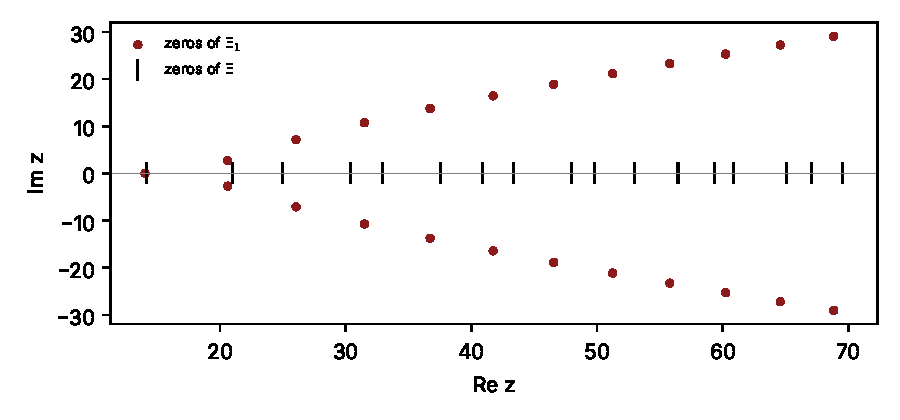
\includegraphics[width=0.85\textwidth]{fig/v3/mh_haglund_zeros.pdf}
\caption{Zeros of the first Haglund approximant $\Xi_1$ (dots) and of $\Xi$ (ticks).}\label{mh:fig:zeros}
\end{figure}

\section{Wald couples, van Dantzig pairs and the Thorin form}\label{mh:sec:wald}

The definitions are in Proposition~\ref{c:thm:wald}. A van Dantzig pair is the weaker notion: two characteristic functions with $f(t)g(it)=1$. A Wald couple is a pair $(X,H)$ with $H\ge0$ and $\E e^{\lambda X}\,\E e^{-\lambda^2H/2}=1$. The book's chart is the clock: $T=H/2$ has $\E e^{-uT}=\xi(\tfrac12)/\xi(\tfrac12+\sqrt u)$ with $u=\lambda^2$, and the Thorin measure of $T$ is $U_{1/2}=\sum_{\gamma>0}\delta_{\gamma^2}$ (rates $\gamma^2/2$ in the variable $\lambda^2/2$ for $H$).

For $\Xi$ itself the partner exists with no hypothesis: $T$ is infinitely divisible and self decomposable, $(X/\sqrt2,T)$ is a Wald couple, and $\Xi(0)/\Xi(it)$ is a characteristic function (Proposition~\ref{c:thm:wald} and Theorem~\ref{thm:ch12:idsd}). RH is the statement that $H$ is a generalised gamma convolution, that is, that $T$ has Thorin measure $U_{1/2}$ with real atoms. Under RH and linear independence, $(Z/\sqrt2,C)$, with $Z$ and $C$ of Proposition~\ref{cw:prop:hit}, is another Wald couple.

For the approximants the Thorin form fails, by Theorem~\ref{mi:thm:noproxy}: the function $\Xi_N(0)/\Xi_N(i\sqrt u)=\prod_j(1+u/z_j^2)^{-1}$ has complex $z_j$, so its Thorin measure $\sum_j\delta_{z_j^2}$ has complex atoms. For $\Xi_1$ the atoms are $197.3$, then $418.1\pm111.3i$, and so on (computed). It is not a generalised gamma convolution. Whether $\Xi_1$ has a Wald partner at all, as a positive variable that is not a generalised gamma convolution, we could not decide: a numerical inversion of the Laplace transform for $N=1$, by a residue sum over $35$ poles and by two numerical inversion methods, is positive at every point tested with $x\ge0.02$ (here $x$ is the variable of the density of $H$), and we did not test below $0.02$. Complex zeros rule out the Thorin form only, not a partner.

Mixtures do not inherit couples. If each component had a partner with transform $\varphi_n$, the mixture would need $1/\sum_np_n/\varphi_n$, a harmonic mean of Laplace transforms, which is not completely monotone in general. The positive result in the opposite direction is the subset construction of Section~\ref{ap:sec:law}.

The contrast is P\'olya's approximant, which replaces $\phi_1(|u|)$ by a smooth even kernel of the form $\cosh(\tfrac92u)\exp(-2\pi\cosh2u)$. Its transform is a combination of $K$ Bessel functions with only real zeros \cite{Polya}, and an even entire function of order one with real zeros has the Hadamard product $\prod(1-z^2/z_j^2)$, so the approximant has a generalised gamma convolution partner and a van Dantzig pair. The difference from Haglund is exactly the corner at the origin. Smoothness at $u=0$ is necessary for the Thorin form of an approximant (Theorem~\ref{mi:thm:noproxy}); we do not claim it is sufficient.

\section{What complete monotonicity tolerates}\label{mh:sec:tolerance}

Existence of the partner and its Thorin form are different statements, and the following mechanism shows how far apart they are. One real rate absorbs a complex pair.

\begin{proposition}\label{mh:prop:absorb}
Let $a=A+iB$ with $A>0$ and $B>0$, and let $r>0$. Then
\[
u\mapsto\frac{1}{(1+u/r)(1+u/a)(1+u/\bar a)}
\]
is completely monotone on $u>0$ if and only if $r\le A$.
\end{proposition}

\begin{proof}
The last two factors are the Laplace transform of $k(x)=\frac{|a|^2}{B}e^{-Ax}\sin Bx$, and the first of $re^{-rx}$. Their convolution is
\[r\,\frac{|a|^2}{B}\,e^{-rx}\int_0^xe^{(r-A)y}\sin(By)\,dy.\]
If $r\le A$, $\int_0^x\omega(y)\sin(By)\,dy\ge0$ for every nonincreasing $\omega\ge0$, by the second mean value theorem, so the density is nonnegative and Bernstein's theorem applies. If $r>A$, put $c=r-A>0$. Then $\int_0^{2\pi/B}e^{cy}\sin(By)\,dy=B(1-e^{2\pi c/B})/(c^2+B^2)<0$, and the convolution is negative at $x=2\pi/B$. With no real factor at all the density $k$ itself changes sign.
\end{proof}

Now let $N_0(T)$ count the zeros $\tfrac12+i\gamma$ with $0<\gamma\le T$ (with multiplicity) and $P(T)$ the pairs of zeros $\beta+i\gamma$, $1-\beta+i\gamma$ with $\beta>\tfrac12$, $0<\gamma\le T$, also with multiplicity.

\begin{theorem}\label{mh:thm:tolerance}
If $P(T)\le N_0(T-1)$ for every $T>0$, then $u\mapsto\xi(\tfrac12)/\xi(\tfrac12+\sqrt u)$ is completely monotone.
\end{theorem}

\begin{proof}
By Hadamard's product, with $u=\lambda^2$,
\[
\frac{\xi(\frac12+\lambda)}{\xi(\frac12)}=\prod_{\gamma_j>0}\Big(1+\frac{u}{r_j}\Big)\prod_{\text{pairs}}\Big(1+\frac ua\Big)\Big(1+\frac u{\bar a}\Big),
\]
with $r_j=\gamma_j^2$ over the zeros on the line and $a=\gamma^2-b^2-2ib\gamma$ for a pair with $b=\beta-\tfrac12$ and height $\gamma$. Order both lists by height and match the $m$th pair to the $m$th zero on the line. The hypothesis gives $\gamma_j\le\gamma-1$, so $r_j\le\gamma^2-2\gamma+1\le\gamma^2-\tfrac14\le\Re a$, using $b<\frac12$ and $\gamma\ge\frac58$, and Proposition~\ref{mh:prop:absorb} applies to each matched triple. The product converges absolutely because $\sum|\rho|^{-2}<\infty$, and it has no exponential factor because $\xi(\tfrac12+\lambda)$ is even and of order one. Unmatched factors $(1+u/r_j)^{-1}$ are completely monotone, products of completely monotone functions are completely monotone, and the class is closed under pointwise limits.
\end{proof}

\begin{remark}\label{mh:rem:tolerance}
The partner exists with no hypothesis by Proposition~\ref{c:thm:wald}, so Theorem~\ref{mh:thm:tolerance} is not needed for existence. It records a tolerance: complete monotonicity survives a positive proportion of off line pairs. A statement in terms of a proportion needs a margin. Suppose that for some $\delta>0$ a proportion at least $\frac13+\delta$ of the zeros up to $T$ lie on the line for all $T\ge T_0$. Then $P(T)\le\frac12(N(T)-N_0(T))\le(\frac13-\frac\delta2)N(T)$, while $N_0(T-1)\ge N_0(T)-(N(T)-N(T-1))\ge(\frac13+\delta)N(T)-O(\log T)$, so the hypothesis holds for $T\ge T_1(\delta)$, and for $T<\max(T_0,T_1)$ one needs all zeros on the line. Without the margin the implication fails: a single zero on the line, at height $14$, and one off line pair at height $14.5$ give $P(14.5)=1>N_0(13.5)=0$. Conrey's theorem puts more than two fifths of the zeros on the line \cite{Conrey89}, which is a margin, but $T_1$ is not explicit, and all zeros below $3\times10^{12}$ are on the line \cite{PT21}.

The lesson for the programme is that existence of $H$ is not RH. An off line pair at height $\gamma$ would show up in the density of $T$ as a factor $e^{-Ax}\sin Bx$ with $B/A\approx2b/\gamma$, an oscillation so slow relative to its decay that one real pole below it hides it completely. Complete monotonicity cannot see it. The Thorin measure does: its atoms would sit at $A\pm iB$, off the positive axis. This is why the programme must aim at the Thorin measure, and why criteria of van Dantzig or Wald type alone cannot reach RH, in the sense of the paragraph after Proposition~\ref{c:thm:wald}.
\end{remark}

Conversely, complete monotonicity forces the lowest rate to be real, since the Laplace transform of a positive measure has its first singularity on the real axis; beyond that, Proposition~\ref{mh:prop:absorb} shows only compatibility with complex higher zeros, under the constraint $r\le A$. For Haglund's $\Xi_1$ the theorem does not decide the question, since there is one positive real zero and infinitely many complex pairs; Proposition~\ref{mh:prop:absorb} disposes only of the first pair ($r=197.3\le A=418.1$).

\section{The total positivity ladder}\label{mh:sec:ladder}

Let $f$ be the density of the van Dantzig partner, with characteristic function $\Xi(0)/\Xi(it)$. By Schoenberg's theorem \cite{Schoenberg51} a density is a P\'olya frequency function of every order ($\mathrm{PF}_\infty$) if and only if the reciprocal of its bilateral Laplace transform is in the Laguerre and P\'olya class, so RH holds if and only if $f$ is $\mathrm{PF}_\infty$ (Chapter~\ref{p:ch:path}). Between the partner itself and RH lies the ladder $\mathrm{PF}_1\supset\mathrm{PF}_2\supset\cdots$, with $\mathrm{PF}_1$ the statement $f\ge0$ and $\mathrm{PF}_2$ log concavity. Note that $\mathrm{PF}_1$ is strictly weaker than complete monotonicity of the transform of $H$. The detection of an off line zero by the rungs is Theorem~\ref{p:thm:detect} and Corollary~\ref{p:cor:detect}, with the residue sign rule of Proposition~\ref{p:prop:signrule}, the far field positivity of each rung in Theorem~\ref{p:thm:farpfk}, and a planted failure in the cosine model in Proposition~\ref{e:prop:toy}. Log concavity of $f$ for $\zeta$ is the certified Theorem~\ref{p:thm:m1}. What follows is the Hankel form of the same index rule, with Karlin's derived determinants in place of shifted minors, and a table.

For a finite product $\prod_j(1+t^2/\kappa_j^2)^{-1}$ with distinct rates, $\Re\kappa_j>0$, closed under conjugation, the inverse transform is $f(x)=\sum_jc_je^{-\kappa_jx}$ for $x>0$ (for $\Xi$ itself the series over the zeros diverges for $x<\pi/4$, Chapter~\ref{p:ch:path}, and only the finite expansion with a remainder is available), with rates $\kappa_j=\gamma_j$ for zeros on the line and $\kappa=\gamma_0\mp id$ for an off line pair (offset $d$), ordered by real part, and let
\[
H_r(x)=(-1)^{r(r-1)/2}\det\big[f^{(i+j)}(x)\big]_{0\le i,j<r}.
\]
If $f$ is smooth and $\mathrm{PF}_r$ then the kernel $f(x-y)$ is totally positive of order $r$, and its derived determinants $\det[\partial_x^i\partial_y^jf(x-y)]_{0\le i,j<r}=H_r(x-y)$ are nonnegative \cite{Karlin68}. So $H_r\ge0$ is necessary for $\mathrm{PF}_r$; $H_1=f$ and $H_2=f'^2-ff''$.

\begin{proposition}\label{mh:prop:hankel}
For a finite product with distinct rates,
\[
H_r(x)=(-1)^{r(r-1)/2}\sum_{|S|=r}\prod_{j\in S}c_je^{-\kappa_jx}\prod_{i<j\in S}(\kappa_i-\kappa_j)^2.
\]
Hence, as $x\to\infty$, if $\kappa_r,\kappa_{r+1}=\gamma_0\mp id$ is a complex pair preceded by $r-1$ real rates below $\gamma_0$, and $\Re\kappa_{r+2}>\gamma_0$, $H_r(x)$ is asymptotic to a positive multiple of $e^{-(\kappa_1+\cdots+\kappa_{r-1}+\gamma_0)x}\cos(dx+\varphi)$ and changes sign infinitely often, with gaps tending to $\pi/d$. If the first $r$ rates are closed under conjugation and $\Re\kappa_r<\Re\kappa_{r+1}$, then $H_r(x)>0$ for large $x$.
\end{proposition}

\begin{proof}
$f^{(n)}=\sum_jc_j(-\kappa_j)^ne^{-\kappa_jx}$, so the Hankel matrix is $V^{\!\top}DV$ with $V$ a Vandermonde matrix in $-\kappa_j$, and the formula is Cauchy and Binet. The sign of the residues $c_j$ is the rule of Proposition~\ref{p:prop:signrule}: for a real rate, $c_j$ has the sign $(-1)^{n_j}$, $n_j$ the number of real rates below $\kappa_j$, because a complex pair contributes a positive factor. So for $S=\{1,\dots,r\}$ with real rates the product has sign $(-1)^{r(r-1)/2}$ and this subset dominates, which is the far field positivity of Theorem~\ref{p:thm:farpfk}. With a complex pair in slots $r,r+1$ the two leading subsets are conjugate, which gives the oscillation. If the first $r$ rates are closed under conjugation, each pair among them contributes $|c|^2(\kappa-\bar\kappa)^2=-4d^2|c|^2$, the sign two real rates would give.
\end{proof}

A computation with the first $60$ zeros, in which zeros $m$ and $m+1$ are replaced by a pair at their midpoint with offset $d$, gives the signs below on the grid $1\le x\le40$, step $0.25$, for $r\le5$. The signs are certified (ball arithmetic at 4000 bits, the sixty zeros taken as exact inputs; no ball was undecided) for this model, which is not $\zeta$ itself.

\begin{table}[ht]
\centering\footnotesize\setlength{\tabcolsep}{4pt}
\begin{tabular}{lccccc}
\toprule
planted pair & $H_1$ & $H_2$ & $H_3$ & $H_4$ & $H_5$\\
\midrule
none & $+$ & $+$ & $+$ & $+$ & $+$\\
$m=1$, $d=0.5$ & $-$ at $7.0$ & $+$ & $+$ & $+$ & $+$\\
$m=2$, $d=0.5$ & $+$ & $-$ at $7.0$ & $+$ & $+$ & $+$\\
$m=3$, $d=0.5$ & $+$ & $+$ & $-$ at $7.25$ & $+$ & $+$\\
$m=4$, $d=0.5$ & $+$ & $+$ & $+$ & $-$ at $7.5$ & $+$\\
$m=5$, $d=0.5$ & $+$ & $+$ & $+$ & $+$ & $-$ at $7.5$\\
$m=2$, $d=0.1$ & $+$ & $-$ at $32.25$ & $+$ & $+$ & $+$\\
$m=3$, $d=0.1$ & $+$ & $+$ & $-$ at $32.5$ & $+$ & $+$\\
\bottomrule
\end{tabular}
\caption{Planted off line pairs and the Hankel determinants $H_r$. A minus sign marks the first $x$ at which $H_r<0$ on the grid; every other entry is positive on the whole grid.}\label{mh:tab:planted}
\end{table}

For small $d$ the pair term is close to that of a double pole, proportional to $\sin(dx)/d$, so one expects the first sign change near $x=\pi/d$ ($6.3$ and $31.4$): the computed first changes are $7.0$ to $7.5$ and $32.25$ to $32.5$. In the table a pair in slots $m,m+1$ is first detected by the Hankel determinant of order $m$, at distance $x\approx\pi/d$, where $f$ is of size $e^{-\gamma_1\pi/d}$; the lower orders stay positive on the grid, which Proposition~\ref{mh:prop:hankel} does not guarantee in general. This is the index rule of Theorem~\ref{p:thm:detect}, seen here for the finite product.

\begin{remark}\label{mh:rem:ladder}
Proposition~\ref{mh:prop:hankel} is a statement about $x\to\infty$ for a finite product, a far field statement. It does not show that $\mathrm{PF}_r$ holds for all $x$ when the first $r$ zeros are real, and it does not make $\mathrm{PF}_r$ a statement about the first $r$ zeros only: log concavity of $f$ is a global condition to which every zero contributes in the near field, and by Table~\ref{mh:tab:planted} the determinant $H_2$ already detects the pair in slots $2$ and $3$. For $\zeta$ log concavity is certified, Theorem~\ref{p:thm:m1}. The theorems of Chapter~\ref{p:ch:path} decide each fixed configuration only for $x$ large enough, not uniformly in the configuration. We verified only the Hankel conditions $H_r$, which are necessary for $\mathrm{PF}_r$, not $\mathrm{PF}_r$ itself. No finite rung reaches RH; RH is uniformity in $r$. The Thorin measure is the object at $r=\infty$: it lists every rate at once.
\end{remark}

\section{A statistical form of the sequence and the cancellation of kinks}\label{mh:sec:cancel}

Let $K(\lambda)=\log\xi(\tfrac12+\lambda)-\log\xi(\tfrac12)$, the cumulant generating function of the P\'olya law, so that $G(\tfrac12+\lambda)=K'(\lambda)$ is the mean of the law tilted by $e^{\lambda u}$ and $K^{(m)}(\lambda)$ its $m$th cumulant. By the Curry and Schoenberg form of a divided difference \cite{CurrySchoenberg66},
\[
g_k=(-2)^k\,\E\,K^{(k+1)}\big(\tfrac32+2S_k\big),\qquad S_k=U_1+\cdots+U_k,
\]
with $U_i$ independent uniforms on $(0,1)$ (checked at $k=2$ to fifteen digits, computed). So $g_k$ is $(-2)^k$ times the cumulant of order $k+1$ of the tilted P\'olya law, averaged over a B spline of tilts on $[\tfrac32,\tfrac32+2k]$, and Theorem~\ref{mh:thm:landau} says: RH holds if and only if $(-1)^k\E K^{(k+1)}(\tfrac32+2S_k)\le C2^{-k}k^{-3/4}$, equivalently the lower bound. The Keiper and Li coefficients of Section~\ref{ch:li} are the analogous quantities at the tilt $\frac12$, and Li's criterion \cite{Li97} is likewise one sided. They are combinations of several derivatives of $\log\xi$ at $s=1$, not a single cumulant, so the analogy is loose.

All odd derivatives of the even smooth kernel $\Phi$ vanish at the origin. So for every $m\ge0$
\[
\sum_{n\ge1}\phi_n^{(2m+1)}(0)=0,
\]
and with $\kappa_N^{(m)}=\sum_{n\le N}\phi_n^{(2m+1)}(0)=-\sum_{n>N}\phi_n^{(2m+1)}(0)$, so that $\kappa_N=\kappa_N^{(0)}$, the expansion of Remark~\ref{mh:rem:kink} gives $\Xi_N(t)\sim\sum_m(-1)^{m+1}4\kappa_N^{(m)}t^{-2m-2}$: its coefficients are the tails of these sums. The functional equation is this infinite family of cancellations across the mixture index; for $m=0$ it is the kink identity of Lemma~\ref{mi:lem:kink}. A Beurling system has the positivity ($\Lambda\ge0$) but no such family. Heuristically, positivity without cancellation is not enough: the single component $\phi_1$ is positive, and its transform has one positive real zero, which we computed for $n=1$ only. RH lives where positivity and cancellation hold together.

Is there a path here? Not yet, but the requirement is concrete. One needs an argument in which the positivity $\phi_n\ge0$ of each component and the cancellation $\sum_n\phi_n^{(2m+1)}(0)=0$ are used jointly to produce the one sided bound of Theorem~\ref{mh:thm:landau}. Neither the $2\sin^2$ lemma, which sees only positivity, nor term by term analysis of the incomplete gamma functions, which sees only one $n$, can do it alone.

The zero sum form of the Maslanka sequence of $\xi$, Theorem~\ref{mh:thm:landau}, the mixture form, the tolerance mechanism and the planted pair table are from an unrefereed note of Polson (November 2026). The kink theorem, the real zero counts of Haglund's approximants and the index rule for detection are results of Chapter~\ref{ch:miyatake} and Chapter~\ref{p:ch:path}, quoted above, and Haglund's own observations and conjectures \cite{Haglund09} are quoted, not checked by us.

\paragraph{Open problems.}
\begin{enumerate}
\item Decide whether $\Xi_1(0)/\Xi_1(i\sqrt u)$ is completely monotone, that is, whether the approximant $\Xi_1$ has a Wald partner.
\item Smooth the corner: find a positive mixture representation of $\Phi$ whose components are even and smooth and have transforms with only real zeros, so that each has a generalised gamma convolution partner (smoothness alone does not suffice: an equal mixture of two centred normal laws has a characteristic function with nonreal zeros). Williams's Gamma(2) representation and the ferromagnetic families of Chapter~\ref{chap:ferro} are candidates.
\item Express $g_k$, or $R_k$, directly through the $\phi_n$ and the kink sums, and look for the sign of Theorem~\ref{mh:thm:landau} there.
\item Find an inductive step on the total positivity ladder: from $\mathrm{PF}_r$ and the functional equation to $\mathrm{PF}_{r+1}$.
\item Track the complex atoms $z_j^2$ of $\Xi_N$ as $N$ grows, and test in that variable Haglund's conjecture on the ordering of the zeros of each $\Xi_N$ \cite{Haglund09}.
\end{enumerate}
